\documentclass[11pt,aspectratio=169,usenames,dvipsnames]{beamer}
%\beamerdefaultoverlayspecification{<+->}
\usefonttheme[onlymath]{serif}
%\usetheme{Madrid}
%\usetheme{metropolis}

\usetheme{Madrid}
\usetheme[subsectionpage=progressbar]{metropolis} 

\usepackage[utf8]{inputenc}
\usepackage{amsmath,bbding}
\usepackage{amsfonts}
\usepackage{amssymb}
\usepackage{subfig}
\usepackage{colortbl}
\usepackage{xcolor}
\definecolor{myorange}{HTML}{f07e26}
% \usepackage{tabularx}

%\author{\textbf{Mostafa Sadeghi}\\
%Perception team, INRIA Grenoble Rh\^one-Alpes, France\\}
%%\title{Deep Latent Variable Generative Models: Application to Audio-visual Speech Enhancement}
%
%\title{Unsupervised Audio-visual Speech Enhancement based on Variational Autoencoders}
%
%%\addtobeamertemplate{navigation symbols}{}{%
%%\usebeamerfont{footline}%
%%\usebeamercolor[fg]{footline}%
%%\hspace{1em}%
%%\insertframenumber/\inserttotalframenumber
%%}

% logos for the first frame
% \titlegraphic{%
% 	%  \includegraphics[width=.2\textwidth]{example-image-a}\hfill
% 	%  \includegraphics[width=.2\textwidth]{example-image-b}\hfill
% 	\includegraphics[width=.2\textwidth]{logos/inriaLogo} \hfill \includegraphics[width=.12\textwidth]{logos/logo-uga.png} \hfill \includegraphics[width=.07\textwidth]{logos/logo-ljk.png} \hfill \includegraphics[scale=0.23]{logos/miaiLogo}  %\includegraphics[scale=0.13]{logo_gipsa-lab.png}
% }

% first frame
\makeatletter

\setbeamertemplate{title page}{
	\begin{minipage}[b][\paperheight]{\textwidth}
		\centering
		\vfill%
		\ifx\inserttitle\@empty\else\usebeamertemplate*{title}\fi
		\ifx\insertsubtitle\@empty\else\usebeamertemplate*{subtitle}\fi
		\usebeamertemplate*{title separator}
		\ifx\beamer@shortauthor\@empty\else\usebeamertemplate*{author}\fi
		\ifx\insertinstitute\@empty\else\usebeamertemplate*{institute}\fi
		\vfill
		\ifx\inserttitlegraphic\@empty\else\inserttitlegraphic\fi
		\vspace*{0.25cm}
	\end{minipage}
}
\setbeamertemplate{title}{
	%  \raggedright%
	\linespread{1.0}%
	\inserttitle% 
	\par%
	\vspace*{0.5em}
}
\setbeamertemplate{subtitle}{
	%  \raggedright%
	\insertsubtitle%
	\par%
	\vspace*{0.5em}
}
\makeatother

\setbeamerfont{title}{size=\Large}
\setbeamerfont{author}{size=\small}
\setbeamerfont{institute}{size=\scriptsize}

\author{Generative Multimodal AI\\ Master MoSIG/MSIAM/AI}
\title{Audio representation (learning)}

\institute{Xavier Alameda-Pineda (Xavi)}

\newcommand{\E}{\mathbb{E}}
\usepackage{multimedia}
\usepackage{animate}
\usepackage{hyperref}
\usepackage{tikz}
\usepackage{math}
\usepackage{makecell}
\usepackage{booktabs}
\usepackage{multirow}

%\setbeamertemplate{navigation symbols}{}
%\setbeamertemplate{footline}[page number]{}s
\makeatletter
\let\save@measuring@true\measuring@true
\def\measuring@true{%
  \save@measuring@true
  \def\beamer@sortzero##1{\beamer@ifnextcharospec{\beamer@sortzeroread{##1}}{}}%
  \def\beamer@sortzeroread##1<##2>{}%
  \def\beamer@finalnospec{}%
}
\makeatother
\newcommand{\bs}{\boldsymbol}
\date{March 19, 2020}
%\DeclareMathOperator*{\argmax}{arg\max}

\usepackage[many]{tcolorbox}   

\newtcolorbox{mybox2}[1]{%
	tikznode boxed title,
	enhanced,
	arc=3mm,
	interior style={white},
	attach boxed title to top center= {yshift=-\tcboxedtitleheight/2},
	%    fonttitle=\bfseries,
	colbacktitle=white,
	coltitle=black,
	boxed title style={size=normal,colframe=white,boxrule=0pt}, 
	left=1mm, 
	right=1mm, 
	top=3mm, 
	bottom=2mm, 
	nobeforeafter,
	boxrule=.2mm,
	title={#1}
}

\newcommand\blfootnote[1]{%
	\begingroup
	\renewcommand\thefootnote{}\footnote{\scriptsize #1}%
	\addtocounter{footnote}{-1}%
	\endgroup
}

\setbeamertemplate{footline}{
	\usebeamercolor[fg]{page number in head}%
	\usebeamerfont{page number in head}%
	\begin{flushright}
	\insertframenumber$\quad$
	\end{flushright}\vspace{-2mm}
}

\newcommand{\argmax}{\operatornamewithlimits{argmax}}
\newcommand{\argmin}{\operatornamewithlimits{argmin}}

% \usepackage{tikz}
\usepackage{xstring}

\usetikzlibrary{bayesnet,calc}
\usetikzlibrary{shapes.geometric}
\tikzset{  net/.style={draw,trapezium,trapezium angle=75,shape border rotate=270} }
\tikzset{  rnn/.style={draw,rectangle} }
\usetikzlibrary{fit,positioning}
\newcommand{\drawNodes}[2]{}
\newcommand{\denselyConnectNodes}[2]{}

\newcommand{\mylz}{{\color{red}z}}
\newcommand{\myox}{{\color{green}x}}
\newcommand{\myls}{{\color{red}s}}
\newcommand{\myos}{{\color{green}s}}
\newcommand{\myov}{{\color{green}v}}

\usepackage{neuralnetwork}


\makeatother
\setbeamertemplate{footline}
{
  \leavevmode%
%   \hbox{%
%   \begin{beamercolorbox}[wd=.4\paperwidth,ht=2.25ex,dp=1ex,center]{author in head/foot}%
%     \usebeamerfont{author in head/foot}\insertshortauthor
%   \end{beamercolorbox}%
%   \begin{beamercolorbox}[wd=.6\paperwidth,ht=2.25ex,dp=1ex,center]{title in head/foot}%
    \usebeamerfont{title in head/foot}\hfill
    \insertframenumber{} / \inserttotalframenumber\hspace*{1ex}
%   \end{beamercolorbox}}%
%   \vskip0pt%
}
\makeatletter
\setbeamertemplate{navigation symbols}{}

\AtBeginSection[]{
  \begin{frame}
  \vfill
  \centering
  \begin{beamercolorbox}[sep=8pt,center,shadow=true,rounded=true]{title}
    \usebeamerfont{title}\insertsectionhead\par%
  \end{beamercolorbox}
  \vfill
  \end{frame}
}

\date{}

\newcommand{\centerimage}[2]{\begin{center}\includegraphics[width=#1\textwidth]{#2}\end{center}}

\begin{document}

% %%%%%%%%%%%%%%%%%%%%%%%%%%%%%%%%%%%%%%%%%%%%%%%%%%%%%%%%%%%%%%
\begin{frame}
  \titlepage
\end{frame}


% %%%%%%%%%%%%%%%%%%%%%%%%%%%%%%%%%%%%%%%%%%%%%%%%%%%%%%%%%%%%%%
% Classic representations
% %%%%%%%%%%%%%%%%%%%%%%%%%%%%%%%%%%%%%%%%%%%%%%%%%%%%%%%%%%%%%%
\section{Representing Audio Data}

% %%%%%%%%%%%%%%%%%%%%%%%%%%%%%%%%%%%%%%%%%%%%%%%%%%%%%%%%%%%%%%
\begin{frame}{The raw data}
  \begin{columns}
    \begin{column}{0.4\textwidth}
        Microphones capture the air pressure variations.\vspace{3mm}
        
        This \textit{continuous} signal is \textit{sampled} into a \textit{discrete} signal.\vspace{3mm}

        We never work with $S(t)$ but rather with $S[i]=S_i=S(t=iT)$, where $T$ is the sampling period.

    \end{column}
    \begin{column}{0.6\textwidth}
        \begin{figure}
        \centering
        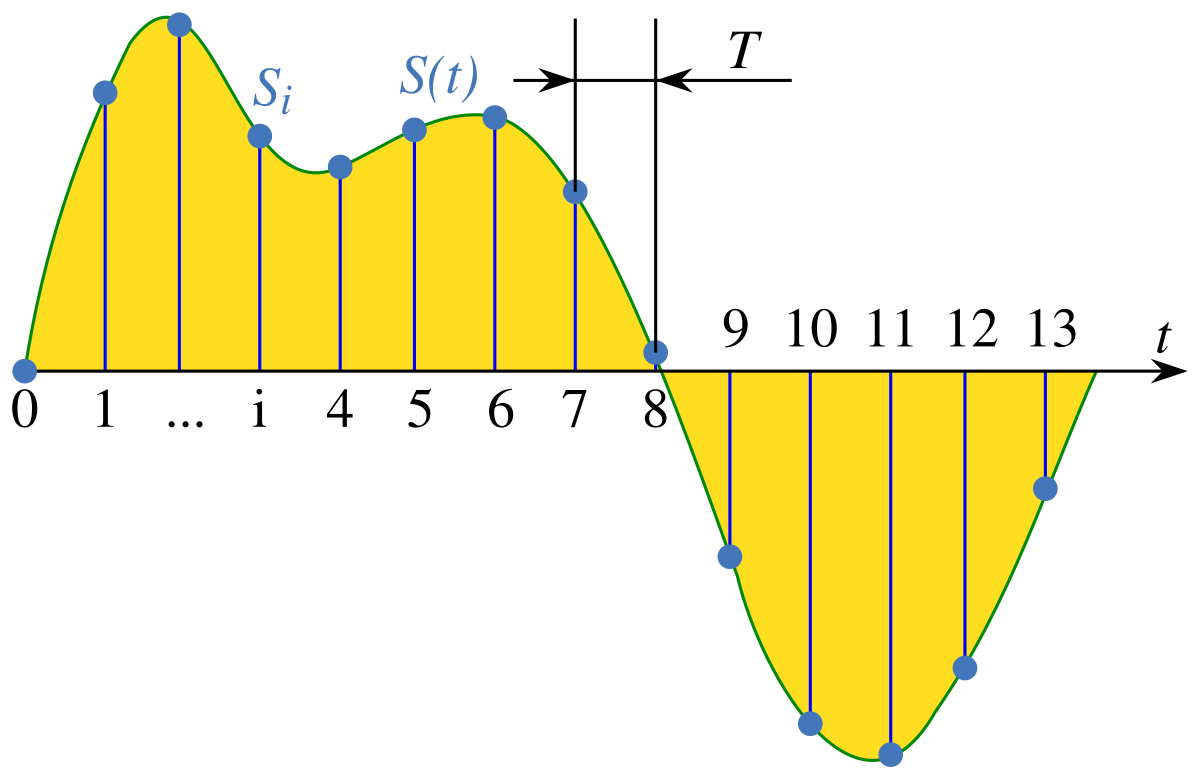
\includegraphics[width=\textwidth]{images/sampling.png}
        \end{figure}
    \end{column}
  \end{columns}
 \end{frame}

% %%%%%%%%%%%%%%%%%%%%%%%%%%%%%%%%%%%%%%%%%%%%%%%%%%%%%%%%%%%%%%
\begin{frame}{The Nyquist frequency}
 What is the problem with sampling?
 \begin{figure}
  \centering
  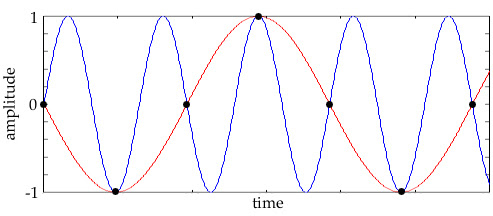
\includegraphics[width=0.65\textwidth]{images/nyquist.jpg}
 \end{figure}
 \textbf{Nyquist-Shanon Sampling Theorem}: If a continuous signal is sampled at a frequency $F_s$, we can only reconstruct the content corresponding to frequencies $<F_s/2$. 
\end{frame}

% %%%%%%%%%%%%%%%%%%%%%%%%%%%%%%%%%%%%%%%%%%%%%%%%%%%%%%%%%%%%%%
\begin{frame}{Every-day example of this}
The phone!
 \begin{itemize}
  \item Speech signal can contain energy up to $20$~kHz.
  \item Most of the energy is within the range $0.3$-$3$~kHz.
  \item This is why the phone standards sample at $8$~kHz.
  \item Keeping most of the content.
  \item Losing high-frequency details - \textit{telephone voice} effect.
 \end{itemize}\vspace{4mm}
\end{frame}

% %%%%%%%%%%%%%%%%%%%%%%%%%%%%%%%%%%%%%%%%%%%%%%%%%%%%%%%%%%%%%%
\begin{frame}{The discrete Fourier transform}
 Purpose: structure the information in frequencies instead of time.\vspace{2mm}\\
 Input: signal in the time domain $s[0],\ldots,s[L-1]$.\vspace{2mm}\\
 Output: a sequence of $L$ complex numbers describing the magnitude and phase at each frequency bin.\vspace{2mm}\\
 Formula: \[S[k] = \sum_{n=0}^{L-1} s[n] \exp\left(-i\frac{2\pi}{L}kn\right).\]
 Fast Fourier transform (FFT): an efficient algorithm to compute DFT when $L$ is a power of 2.
\end{frame}

\begin{frame}{The discrete Fourier transform (II)}
 The signal decomposes in frequencies not in time: either one or the other.\\
 \begin{figure}
  \centering
  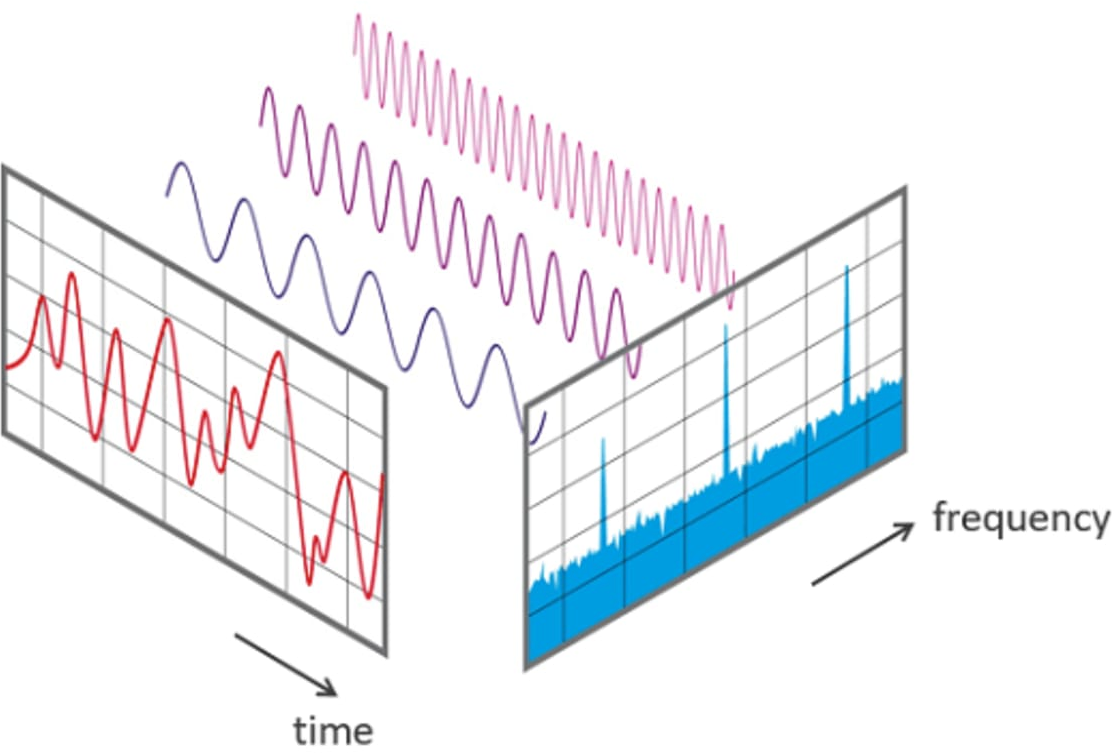
\includegraphics[width=0.6\textwidth]{images/fourierdomain.png}
 \end{figure}
%  Problem: we have to choose either time \textit{or} frequency.
\end{frame}

\begin{frame}{The short-time Fourier transform}
 STFT: segment the input signal, and apply DFT to each segment.
\begin{figure}
\centering
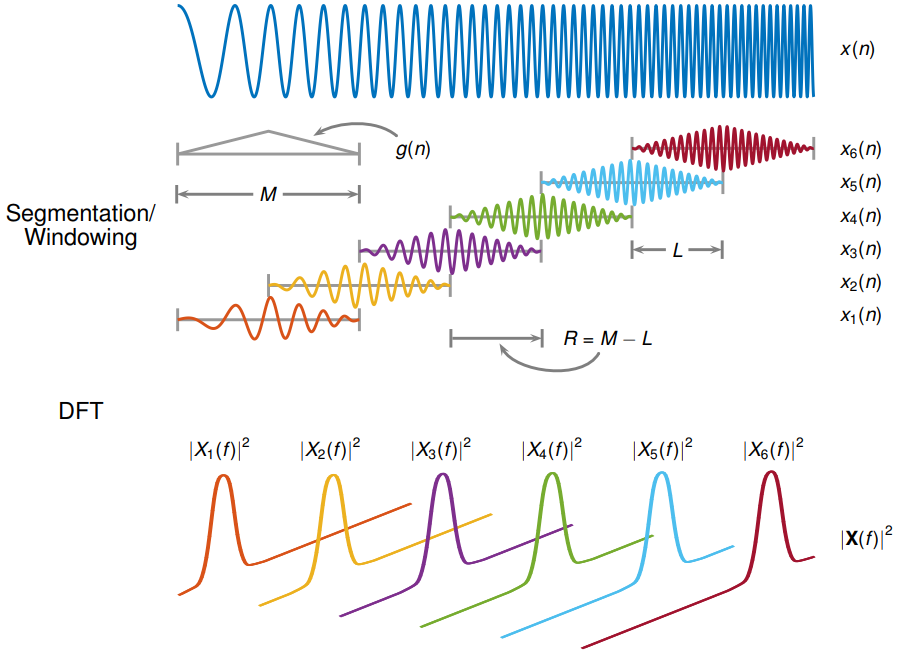
\includegraphics[width=0.6\textwidth]{images/stft.png}
\end{figure}

\alert{Let's check that with a nice wav file!}
\end{frame}

\begin{frame}{STFT comments}
 \begin{itemize}
  \item There is a duality: (i) Represent the frequential content at a given time, (ii) Represent the evolution of a given frequency over time.
  \item STFT requires to \textit{window} the signal with a kernel. Different kernels lead to different properties (e.g.\ reconstruction).
  \item Other parameters: the window length and overlap. They provide the rate of frequency vectors (DFT outputs). If correctly chosen the correspond to, e.g.\ video frames.
 \end{itemize}\vspace{3mm}
 \begin{columns}
    \begin{column}{0.5\textwidth}
        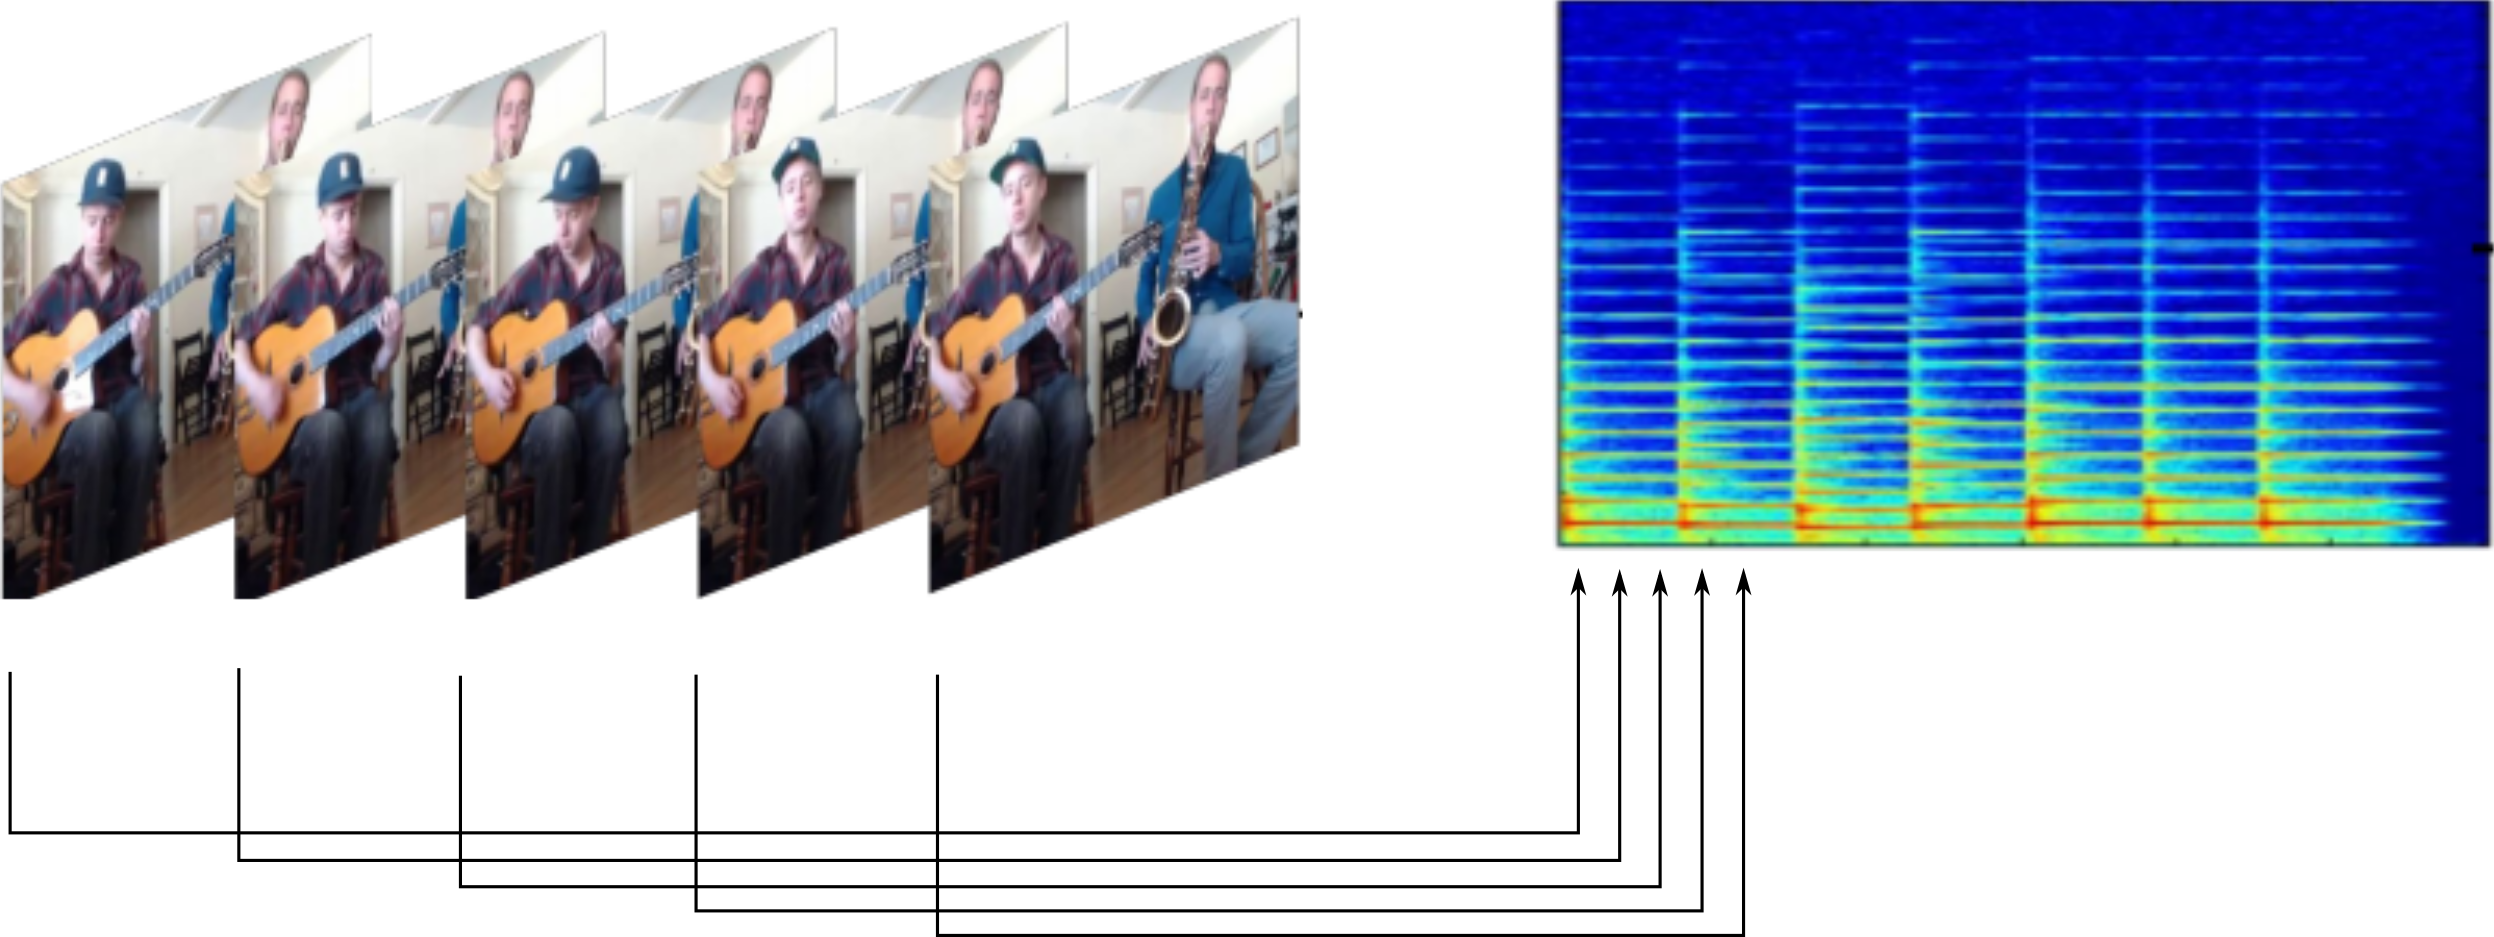
\includegraphics[width=\textwidth]{images/avcorrespondence.png}
    \end{column}
    \begin{column}{0.3\textwidth}
        \centering
        \textcolor{red}{Let's \textit{see} STFTs!}
    \end{column}
 \end{columns}
\end{frame}



\end{document}

